\documentclass{article}\usepackage[]{graphicx}\usepackage[]{xcolor}
% maxwidth is the original width if it is less than linewidth
% otherwise use linewidth (to make sure the graphics do not exceed the margin)
\makeatletter
\def\maxwidth{ %
  \ifdim\Gin@nat@width>\linewidth
    \linewidth
  \else
    \Gin@nat@width
  \fi
}
\makeatother

\definecolor{fgcolor}{rgb}{0.345, 0.345, 0.345}
\newcommand{\hlnum}[1]{\textcolor[rgb]{0.686,0.059,0.569}{#1}}%
\newcommand{\hlstr}[1]{\textcolor[rgb]{0.192,0.494,0.8}{#1}}%
\newcommand{\hlcom}[1]{\textcolor[rgb]{0.678,0.584,0.686}{\textit{#1}}}%
\newcommand{\hlopt}[1]{\textcolor[rgb]{0,0,0}{#1}}%
\newcommand{\hlstd}[1]{\textcolor[rgb]{0.345,0.345,0.345}{#1}}%
\newcommand{\hlkwa}[1]{\textcolor[rgb]{0.161,0.373,0.58}{\textbf{#1}}}%
\newcommand{\hlkwb}[1]{\textcolor[rgb]{0.69,0.353,0.396}{#1}}%
\newcommand{\hlkwc}[1]{\textcolor[rgb]{0.333,0.667,0.333}{#1}}%
\newcommand{\hlkwd}[1]{\textcolor[rgb]{0.737,0.353,0.396}{\textbf{#1}}}%
\let\hlipl\hlkwb

\usepackage{framed}
\makeatletter
\newenvironment{kframe}{%
 \def\at@end@of@kframe{}%
 \ifinner\ifhmode%
  \def\at@end@of@kframe{\end{minipage}}%
  \begin{minipage}{\columnwidth}%
 \fi\fi%
 \def\FrameCommand##1{\hskip\@totalleftmargin \hskip-\fboxsep
 \colorbox{shadecolor}{##1}\hskip-\fboxsep
     % There is no \\@totalrightmargin, so:
     \hskip-\linewidth \hskip-\@totalleftmargin \hskip\columnwidth}%
 \MakeFramed {\advance\hsize-\width
   \@totalleftmargin\z@ \linewidth\hsize
   \@setminipage}}%
 {\par\unskip\endMakeFramed%
 \at@end@of@kframe}
\makeatother

\definecolor{shadecolor}{rgb}{.97, .97, .97}
\definecolor{messagecolor}{rgb}{0, 0, 0}
\definecolor{warningcolor}{rgb}{1, 0, 1}
\definecolor{errorcolor}{rgb}{1, 0, 0}
\newenvironment{knitrout}{}{} % an empty environment to be redefined in TeX

\usepackage{alltt}
\usepackage[sc]{mathpazo}
\renewcommand{\sfdefault}{lmss}
\renewcommand{\ttdefault}{lmtt}
\usepackage[T1]{fontenc}
\usepackage{geometry}
\geometry{verbose,tmargin=2.5cm,bmargin=2.5cm,lmargin=2.5cm,rmargin=2.5cm}
\setcounter{secnumdepth}{2}
\setcounter{tocdepth}{2}
\usepackage[unicode=true,pdfusetitle,
 bookmarks=true,bookmarksnumbered=true,bookmarksopen=true,bookmarksopenlevel=2,
 breaklinks=false,pdfborder={0 0 1},backref=false,colorlinks=false]
 {hyperref}
\hypersetup{
 pdfstartview={XYZ null null 1}}

\makeatletter
%%%%%%%%%%%%%%%%%%%%%%%%%%%%%% User specified LaTeX commands.
\renewcommand{\textfraction}{0.05}
\renewcommand{\topfraction}{0.8}
\renewcommand{\bottomfraction}{0.8}
\renewcommand{\floatpagefraction}{0.75}

\makeatother
\IfFileExists{upquote.sty}{\usepackage{upquote}}{}
\begin{document}








The results below are generated from an R script.

\begin{knitrout}
\definecolor{shadecolor}{rgb}{0.969, 0.969, 0.969}\color{fgcolor}\begin{kframe}
\begin{alltt}
\hlcom{# Question 1}

\hlcom{# Decimal to binary}
\hlcom{# a. 0.625}
\hlcom{# Answer}
\hlcom{# using double dabble method}
\hlcom{# Step 1 multiply by 2 }
\hlcom{# 0.625*2 = 1.25}
\hlcom{# Step 2 if number is larger than 1, put 1 if not put 0.}
\hlcom{# 0.1--}
\hlcom{# use the fractional part of 1.25 and repeat step 1.}
\hlcom{# 0.25*2 = 0.5}
\hlcom{# 0.10-}
\hlcom{# repeat step 1 again to fractional value of 0.5.}
\hlcom{# 0.5*2 = 1}
\hlcom{# 0.101}
\hlcom{# therefore, the decimal value of 0.625 to binary is 0.101 of base 2.}

\hlcom{# b. 1/9 (0.11111...)}
\hlcom{# we only take some decimal place since it is not efficient to show all of the numbers}
\hlcom{# 0.11111*2 = 0.22222 = 0.0-------}
\hlcom{# 0.22222*2 = 0.44444 = 0.00------}
\hlcom{# 0.44444*2 = 0.88888 = 0.000-----}
\hlcom{# 0.88888*2 = 1.77776 = 0.0001----}
\hlcom{# 0.77776*2 = 1.55552 = 0.00011---}
\hlcom{# 0.55552*2 = 1.11104 = 0.000111--}
\hlcom{# 0.11104*2 = 0.22208 = 0.0001110-}
\hlcom{# 0.22208*2 = 0.44416 = 0.00011100}

\hlcom{# we can also keep going since it is repeating, there will be a pattern}
\hlcom{# therefore, the decimal value of 1/9 is 0.00011100 (repeated) of base 2.}

\hlcom{# binary to decimal}
\hlcom{# using positional notation binary}
\hlcom{# the 1 and 0 corresponds if the number has a value or not.}
\hlcom{# if it is 0, the number will be multiplied by 0.}

\hlcom{# a. 1111}
\hlnum{1}\hlopt{*}\hlnum{2}\hlopt{^}\hlnum{3} \hlopt{+} \hlnum{1}\hlopt{*}\hlnum{2}\hlopt{^}\hlnum{2} \hlopt{+} \hlnum{1}\hlopt{*}\hlnum{2}\hlopt{^}\hlnum{1} \hlopt{+} \hlnum{1}\hlopt{*}\hlnum{2}\hlopt{^}\hlnum{0}
\end{alltt}
\begin{verbatim}
## [1] 15
\end{verbatim}
\begin{alltt}
\hlcom{# b. 1010}
\hlnum{1}\hlopt{*}\hlnum{2}\hlopt{^}\hlnum{3} \hlopt{+} \hlnum{0}\hlopt{*}\hlnum{2}\hlopt{^}\hlnum{2} \hlopt{+} \hlnum{1}\hlopt{*}\hlnum{2}\hlopt{^}\hlnum{1} \hlopt{+} \hlnum{0}\hlopt{*}\hlnum{2}\hlopt{^}\hlnum{0}
\end{alltt}
\begin{verbatim}
## [1] 10
\end{verbatim}
\begin{alltt}
\hlcom{# c. 1010.0101}
\hlcom{# write out the integer part first.}
\hlstd{intPart} \hlkwb{=} \hlnum{1}\hlopt{*}\hlnum{2}\hlopt{^}\hlnum{3} \hlopt{+} \hlnum{0}\hlopt{*}\hlnum{2}\hlopt{^}\hlnum{2} \hlopt{+} \hlnum{1}\hlopt{*}\hlnum{2}\hlopt{^}\hlnum{1} \hlopt{+} \hlnum{0}\hlopt{*}\hlnum{2}\hlopt{^}\hlnum{0}
\hlstd{intPart}
\end{alltt}
\begin{verbatim}
## [1] 10
\end{verbatim}
\begin{alltt}
\hlcom{# now write the fractional part (0.0101)}
\hlstd{fracPart} \hlkwb{=} \hlnum{0}\hlopt{*}\hlnum{2}\hlopt{^}\hlstd{(}\hlopt{-}\hlnum{1}\hlstd{)} \hlopt{+} \hlnum{1}\hlopt{*}\hlnum{2}\hlopt{^}\hlstd{(}\hlopt{-}\hlnum{2}\hlstd{)} \hlopt{+} \hlnum{0}\hlopt{*}\hlnum{2}\hlopt{^}\hlstd{(}\hlopt{-}\hlnum{3}\hlstd{)} \hlopt{+} \hlnum{1}\hlopt{*}\hlnum{2}\hlopt{^}\hlstd{(}\hlopt{-}\hlnum{4}\hlstd{)}
\hlstd{fracPart}
\end{alltt}
\begin{verbatim}
## [1] 0.3125
\end{verbatim}
\begin{alltt}
\hlcom{# the answer will be the int + frac which is}
\hlstd{intPart} \hlopt{+} \hlstd{fracPart}
\end{alltt}
\begin{verbatim}
## [1] 10.312
\end{verbatim}
\begin{alltt}
\hlcom{# d. 1.010101...(repeated)}
\hlcom{# do the same as c.}
\hlstd{intPart} \hlkwb{=} \hlnum{1}\hlopt{*}\hlnum{2}\hlopt{^}\hlnum{1}
\hlstd{intPart}
\end{alltt}
\begin{verbatim}
## [1] 2
\end{verbatim}
\begin{alltt}
\hlcom{# fractional part (0.010101)}
\hlstd{fracPart} \hlkwb{=} \hlnum{0}\hlopt{*}\hlnum{2}\hlopt{^}\hlstd{(}\hlopt{-}\hlnum{1}\hlstd{)} \hlopt{+} \hlnum{1}\hlopt{*}\hlnum{2}\hlopt{^}\hlstd{(}\hlopt{-}\hlnum{2}\hlstd{)} \hlopt{+} \hlnum{0}\hlopt{*}\hlnum{2}\hlopt{^}\hlstd{(}\hlopt{-}\hlnum{3}\hlstd{)} \hlopt{+} \hlnum{1}\hlopt{*}\hlnum{2}\hlopt{^}\hlstd{(}\hlopt{-}\hlnum{4}\hlstd{)} \hlopt{+} \hlnum{0}\hlopt{*}\hlnum{2}\hlopt{^}\hlstd{(}\hlopt{-}\hlnum{5}\hlstd{)} \hlopt{+} \hlnum{1}\hlopt{*}\hlnum{2}\hlopt{^}\hlstd{(}\hlopt{-}\hlnum{6}\hlstd{)}
\hlstd{fracPart}
\end{alltt}
\begin{verbatim}
## [1] 0.32812
\end{verbatim}
\begin{alltt}
\hlcom{# add them all to get answer}
\hlstd{intPart} \hlopt{+} \hlstd{fracPart}
\end{alltt}
\begin{verbatim}
## [1] 2.3281
\end{verbatim}
\begin{alltt}
\hlcom{# Question 2 }
\hlcom{# a. 6/7 (0.8571429)}
\hlcom{# 0.8571*2 = 1.7142}
\hlcom{# 0.7142*2 = 1.4284}
\hlcom{# 0.4284*2 = 0.8568}
\hlcom{# 0.8568*2 = 1.7136}
\hlcom{# answer: 0.1101}

\hlcom{# b. 1/7 (0.1428571)}
\hlcom{# 0.1428*2 = 0.2856}
\hlcom{# 0.2856*2 = 0.5712}
\hlcom{# 0.5712*2 = 1.1424}
\hlcom{# 0.1424*2 = 0.2848}
\hlcom{# answer: 0.0010}

\hlcom{# c. }
\hlcom{# 0.1101 + 0.0010 = 0.1111}
\hlnum{1}\hlopt{*}\hlnum{2}\hlopt{^}\hlstd{(}\hlopt{-}\hlnum{1}\hlstd{)} \hlopt{+} \hlnum{1}\hlopt{*}\hlnum{2}\hlopt{^}\hlstd{(}\hlopt{-}\hlnum{2}\hlstd{)} \hlopt{+} \hlnum{1}\hlopt{*}\hlnum{2}\hlopt{^}\hlstd{(}\hlopt{-}\hlnum{3}\hlstd{)} \hlopt{+} \hlnum{1}\hlopt{*}\hlnum{2}\hlopt{^}\hlstd{(}\hlopt{-}\hlnum{4}\hlstd{)}
\end{alltt}
\begin{verbatim}
## [1] 0.9375
\end{verbatim}
\begin{alltt}
\hlcom{# d.}
\hlcom{# 110 (6) +  1 (1) = 111 (7)}
\hlcom{# 111/111 = 1}


\hlcom{# Question 3}
\hlstd{x} \hlkwb{=} \hlnum{1000000}
\hlstd{y} \hlkwb{=} \hlnum{999999}
\hlstd{A} \hlkwb{=} \hlkwa{function}\hlstd{(}\hlkwc{x}\hlstd{,}\hlkwc{y}\hlstd{)\{}
  \hlstd{x}\hlopt{^}\hlnum{4} \hlopt{-} \hlstd{y}\hlopt{^}\hlnum{4}
\hlstd{\}}
\hlstd{B} \hlkwb{=} \hlkwa{function}\hlstd{(}\hlkwc{x}\hlstd{,}\hlkwc{y}\hlstd{)\{}
  \hlstd{(x}\hlopt{^}\hlnum{2}\hlopt{+}\hlstd{y}\hlopt{^}\hlnum{2}\hlstd{)}\hlopt{*}\hlstd{(x}\hlopt{+}\hlstd{y)}\hlopt{*}\hlstd{(x}\hlopt{-}\hlstd{y)}
\hlstd{\}}
\hlkwd{options}\hlstd{(}\hlkwc{digits}\hlstd{=}\hlnum{15}\hlstd{)}
\hlkwd{A}\hlstd{(x,y)}
\end{alltt}
\begin{verbatim}
## [1] 3999993999971581952
\end{verbatim}
\begin{alltt}
\hlkwd{B}\hlstd{(x,y)}
\end{alltt}
\begin{verbatim}
## [1] 3.999994000004e+18
\end{verbatim}
\begin{alltt}
\hlcom{# B is more accurate since R cannot handle big number, and the number x^4 and y^4}
\hlcom{# is very very big.}

\hlcom{# Question 4}
\hlcom{# a. }
\hlcom{# pretend these numbers are prime numbers (1 to 10000 are primes)}
\hlstd{primes} \hlkwb{=} \hlnum{1}\hlopt{:}\hlnum{10000}
\hlcom{# this code will print last 100 elements of this vector}
\hlstd{primes[(}\hlnum{10000}\hlopt{-}\hlnum{100}\hlstd{)}\hlopt{:}\hlnum{10000}\hlstd{]}
\end{alltt}
\begin{verbatim}
##   [1]  9900  9901  9902  9903  9904  9905  9906  9907  9908  9909  9910  9911  9912  9913
##  [15]  9914  9915  9916  9917  9918  9919  9920  9921  9922  9923  9924  9925  9926  9927
##  [29]  9928  9929  9930  9931  9932  9933  9934  9935  9936  9937  9938  9939  9940  9941
##  [43]  9942  9943  9944  9945  9946  9947  9948  9949  9950  9951  9952  9953  9954  9955
##  [57]  9956  9957  9958  9959  9960  9961  9962  9963  9964  9965  9966  9967  9968  9969
##  [71]  9970  9971  9972  9973  9974  9975  9976  9977  9978  9979  9980  9981  9982  9983
##  [85]  9984  9985  9986  9987  9988  9989  9990  9991  9992  9993  9994  9995  9996  9997
##  [99]  9998  9999 10000
\end{verbatim}
\begin{alltt}
\hlcom{#b. }
\hlcom{#this code will add up first 9000 numbers in vector primes.}
\hlkwd{sum}\hlstd{(primes[}\hlnum{1}\hlopt{:}\hlnum{9000}\hlstd{])}
\end{alltt}
\begin{verbatim}
## [1] 40504500
\end{verbatim}
\begin{alltt}
\hlcom{# Question 5.}
\hlstd{x} \hlkwb{=} \hlnum{100}
\hlstd{y} \hlkwb{=} \hlnum{99}
\hlstd{myfunc} \hlkwb{=} \hlkwa{function}\hlstd{(}\hlkwc{x}\hlstd{,}\hlkwc{y}\hlstd{)\{}
  \hlstd{(x}\hlopt{^}\hlnum{16}\hlstd{)}\hlopt{*}\hlstd{(((x}\hlopt{^}\hlnum{8} \hlopt{-} \hlstd{y}\hlopt{^}\hlnum{8}\hlstd{)} \hlopt{/} \hlstd{((}\hlnum{196059601}\hlstd{)}\hlopt{*}\hlstd{(}\hlnum{19801}\hlstd{)}\hlopt{*}\hlstd{(}\hlnum{199}\hlstd{)))} \hlopt{-} \hlnum{1}\hlstd{)}

\hlstd{\}}
\hlkwd{myfunc}\hlstd{(x,y)}
\end{alltt}
\begin{verbatim}
## [1] 133226762955018784
\end{verbatim}
\begin{alltt}
\hlcom{# Question 6}
\hlcom{# to approach this we can use the as.Date library.}
\hlstd{tom} \hlkwb{=} \hlkwd{as.Date}\hlstd{(}\hlstr{"1999-07-05"}\hlstd{)}
\hlstd{david} \hlkwb{=} \hlkwd{as.Date}\hlstd{(}\hlstr{"2003-12-12"}\hlstd{)}

\hlkwd{difftime}\hlstd{(david, tom,} \hlkwc{units} \hlstd{=} \hlstr{"days"}\hlstd{)}
\end{alltt}
\begin{verbatim}
## Time difference of 1621 days
\end{verbatim}
\begin{alltt}
\hlcom{# 7.}
\hlstd{cities} \hlkwb{=} \hlkwd{c}\hlstd{(}\hlstr{"ThunderBay"}\hlstd{,} \hlstr{"Sudbury"}\hlstd{,} \hlstr{"Windsor"}\hlstd{,} \hlstr{"London"}\hlstd{,} \hlstr{"Toronto"}\hlstd{,} \hlstr{"Ottawa"}\hlstd{)}
\hlstd{inc} \hlkwb{=} \hlkwd{c}\hlstd{(}\hlnum{93.07}\hlstd{,} \hlnum{66.79}\hlstd{,} \hlnum{70.16}\hlstd{,} \hlnum{67.22}\hlstd{,} \hlnum{75.24}\hlstd{,} \hlnum{72.96}\hlstd{)}

\hlstd{income} \hlkwb{=} \hlkwd{matrix}\hlstd{(inc,} \hlkwc{nrow} \hlstd{=} \hlnum{1}\hlstd{,} \hlkwc{ncol} \hlstd{=} \hlkwd{length}\hlstd{(cities))}
\hlkwd{colnames}\hlstd{(income)} \hlkwb{<-} \hlstd{cities}

\hlstd{income}
\end{alltt}
\begin{verbatim}
##      ThunderBay Sudbury Windsor London Toronto Ottawa
## [1,]      93.07   66.79   70.16  67.22   75.24  72.96
\end{verbatim}
\begin{alltt}
\hlkwd{barplot}\hlstd{(income,} \hlkwc{ylim} \hlstd{=} \hlkwd{c}\hlstd{(}\hlnum{0}\hlstd{,}\hlnum{100}\hlstd{),} \hlkwc{main} \hlstd{=} \hlstr{"2009 Family Income in Six Cities"}\hlstd{)}
\end{alltt}
\end{kframe}

{\centering 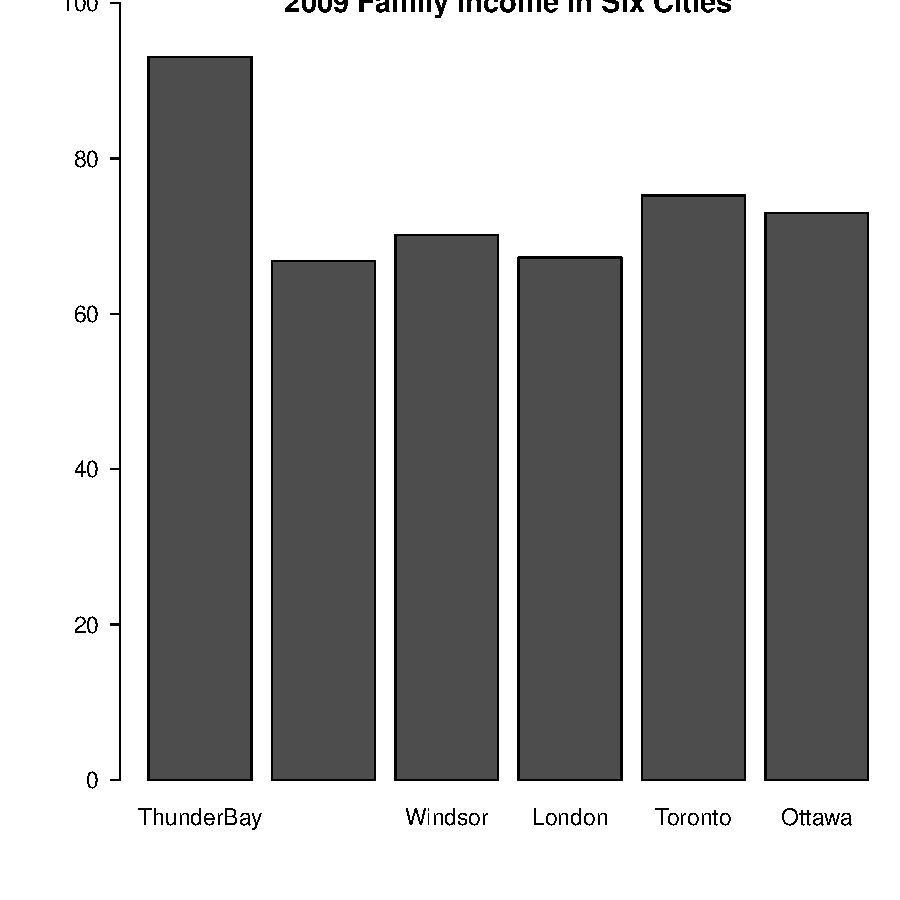
\includegraphics[width=.6\linewidth]{figure/Meng51940633A3-Rnwauto-report-1} 

}


\begin{kframe}\begin{alltt}
\hlkwd{dotchart}\hlstd{(income,} \hlkwc{labels} \hlstd{=} \hlstr{""}\hlstd{,} \hlkwc{xlim} \hlstd{=} \hlkwd{c}\hlstd{(}\hlnum{35}\hlstd{,}\hlnum{100}\hlstd{),} \hlkwc{main} \hlstd{=} \hlstr{"2009 Family Income in Six Cities"}\hlstd{)}
\end{alltt}
\end{kframe}

{\centering 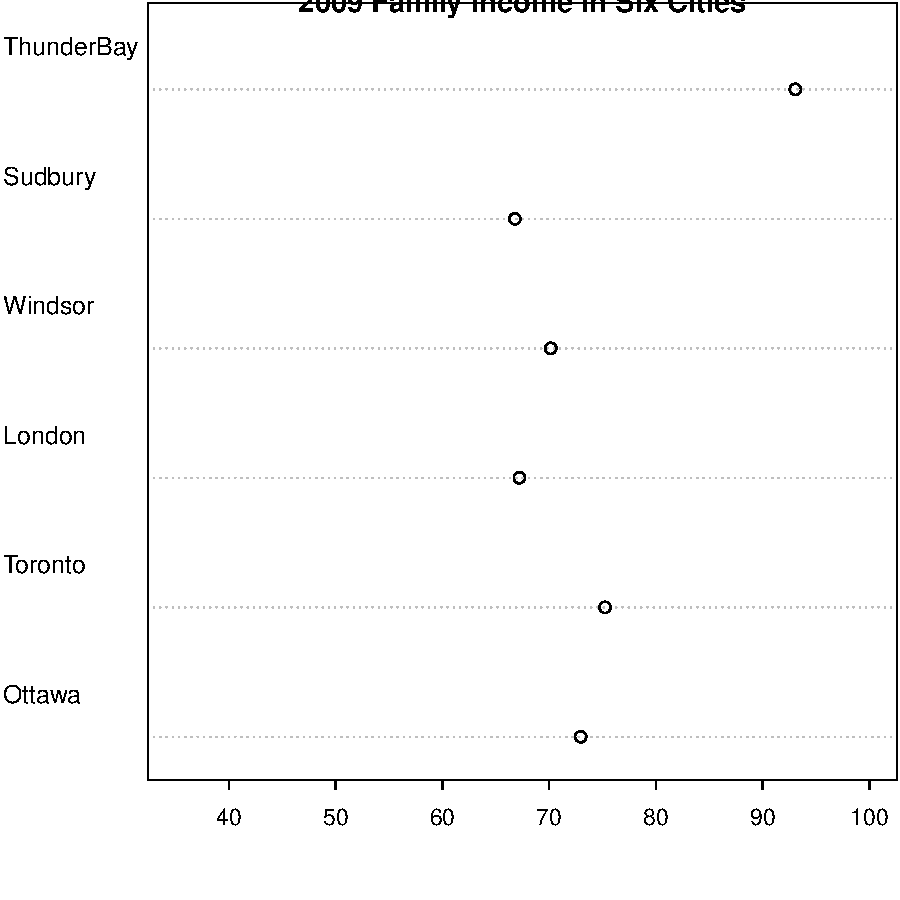
\includegraphics[width=.6\linewidth]{figure/Meng51940633A3-Rnwauto-report-2} 

}


\end{knitrout}

The R session information (including the OS info, R version and all
packages used):

\begin{knitrout}
\definecolor{shadecolor}{rgb}{0.969, 0.969, 0.969}\color{fgcolor}\begin{kframe}
\begin{alltt}
\hlkwd{sessionInfo}\hlstd{()}
\end{alltt}
\begin{verbatim}
## R version 4.2.2 (2022-10-31 ucrt)
## Platform: x86_64-w64-mingw32/x64 (64-bit)
## Running under: Windows 10 x64 (build 19044)
## 
## Matrix products: default
## 
## locale:
## [1] LC_COLLATE=English_United States.utf8  LC_CTYPE=English_United States.utf8   
## [3] LC_MONETARY=English_United States.utf8 LC_NUMERIC=C                          
## [5] LC_TIME=English_United States.utf8    
## 
## attached base packages:
## [1] stats     graphics  grDevices utils     datasets  methods   base     
## 
## loaded via a namespace (and not attached):
## [1] compiler_4.2.2 tools_4.2.2    tinytex_0.44   highr_0.10     knitr_1.42    
## [6] xfun_0.37      evaluate_0.20
\end{verbatim}
\begin{alltt}
\hlkwd{Sys.time}\hlstd{()}
\end{alltt}
\begin{verbatim}
## [1] "2023-02-25 19:56:43 PST"
\end{verbatim}
\end{kframe}
\end{knitrout}


\end{document}
